
%     %%%%%%%%%%%%%%%
%
%     P A C K A G E S
%
%     %%%%%%%%%%%%%%%

\documentclass[11pt, a4paper]{article}
\usepackage{fontspec}
\usepackage{caption}
\usepackage{mathtools}
\usepackage{gensymb}

% DOCUMENT LAYOUT
\usepackage{geometry}
\geometry{a4paper, textwidth=42em, textheight=70em, marginparsep=0.5em, marginparwidth=3.5em}
\setlength\parindent{0em}
\setlength\parskip{0.75em}
\captionsetup{width=0.8\textwidth}

% FONTS
\usepackage[usenames,dvipsnames]{xcolor}
\usepackage{xunicode}
\usepackage{xltxtra}
\defaultfontfeatures{Mapping=tex-text}
%\setromanfont [Ligatures={Common}, Numbers={OldStyle}, Variant=01]{Linux Libertine O}
%\setmonofont[Scale=0.8]{Monaco}
%%% modified by Karol Kozioł for ShareLaTeX use
\setmainfont[
  Ligatures={Common}, Numbers={OldStyle}, Variant=01,
  BoldFont=LinLibertine_RB.otf,
  ItalicFont=LinLibertine_RI.otf,
  BoldItalicFont=LinLibertine_RBI.otf
]{LinLibertine_R.otf}
\setmonofont[Scale=0.8]{DejaVuSansMono.ttf}

% HEADINGS
\usepackage{sectsty}
\usepackage[normalem]{ulem}
\sectionfont{\mdseries\upshape\Large}
\subsectionfont{\mdseries\scshape\normalsize}
\subsubsectionfont{\mdseries\upshape\normalsize}

\renewenvironment{abstract}{%
{\mdseries\scshape\Large\abstractname}
\vspace{1em}\\
}{\par\noindent}


\usepackage[superscript]{cite}

% LISTINGS
\usepackage{listings}
\usepackage{color}
\usepackage{appendix}

\usepackage{color}
\definecolor{codered}{rgb}{0.61,0.21,0.18}
\definecolor{codegreen}{rgb}{0,0.6,0}
\definecolor{codegray}{rgb}{0.5,0.5,0.5}
\definecolor{codepurple}{rgb}{0.58,0,0.82}
\definecolor{backcolour}{rgb}{1.0,1.0,1.0}
\lstset{
  backgroundcolor=\color{backcolour},   
  commentstyle=\color{codegray},
  keywordstyle=\color{codered},
  numberstyle=\tiny\color{codegreen},
  stringstyle=\color{codepurple},
  basicstyle=\footnotesize\ttfamily,        % the size of the fonts that are used for the code
  breaklines=true,                          % sets automatic line breaking
  keepspaces=true,                          % keeps spaces in text, useful for keeping indentation of code
  showspaces=false,                         % show spaces everywhere adding particular underscores; it overrides 'showstringspaces'
  showstringspaces=false,                   % underline spaces within strings only
  showtabs=false,                           % show tabs within strings adding particular underscores
  stepnumber=2,                             % the step between two line-numbers. If it's 1, each line will be numbered
  tabsize=4, 	                            % sets default tabsize to 2 spaces
  title=\lstname                            % show the filename of files included with \lstinputlisting
}


%     %%%%%%%%%%%%%%%
%
%     D O C U M E N T
%
%     %%%%%%%%%%%%%%%


\begin{document}
\title{IAR Task 2 Report}
\author{Angus Pearson -- s1311631\\ Jevgenij Zubovskij -- s1346981}
\date{\today}
\maketitle

%       ^v^v^v^v^v^v^v^v^v^v^v^v^v^v^v^v^v^v^v^v^v^v^v^v^v^v^v^v^v^v^v^v^v^v^v^


\begin{abstract}
  % TODO : Maybe do more experiments?

  %ANGUS - atop, I drew a diaram where  I call it hybryd subsumptions etc, need t odiscuss
  %TODO define our arhcitecture name
  We present an implementation of an algorithm similar to \textit{Bug2} \cite{principlesrobot} 
  built atop reactive obstacle collision avoidance and edge following behaviour developed for 
  \textit{Task1} with the \textit{Khepera} robot. The existing architecture is extended to
  include storing and publishing timestamped poses and goal states in a Redis \cite{Redis} server.
  Real-time visualisation using a Redis to ROS \cite{ROS} pipe provides a graphical display 
  of odometry, sensory information and goals in Rviz. After-the-fact plotting is provided 
  with MatPlotLib independent of ROS.
	
  %TODO update numbers everywhere
  In our testing, the robot was able to navigate to within 10cm of the origin (it's start point) 
  from an abitary location in multiple environments successfully in 12/15 experiments, where each 
  environment was designed to evoke edge-case behaviour considered hard for the algorithm. The 
  algorithm performs comparably in a static world and a dynamic one in which other actors 
  (e.g. Humans) present a transient obstacle. 
\end{abstract}

%       ^v^v^v^v^v^v^v^v^v^v^v^v^v^v^v^v^v^v^v^v^v^v^v^v^v^v^v^v^v^v^v^v^v^v^v^


\section{Introduction}
\label{Introduction}

The second IAR assignment entails extending the existing systems from Task 1 with Odometry, 
to maintain an estimate of the robot's location, enabling rendering of it's movement both 
in real time and after reaching the goal. The task also calls for `return to home' ability, 
``either by retracing its outward route or more directly''. As an extention, basic mapping 
of the world is desireable (without localisation correction for odometry dead-reckoning drift). 

The navigational behaviour we have developed is bolted-on to the simpler reactive wall-following
and collision avoidance code we have from \textit{Task1}, in a hybrid-subsumtive sense where the
higher-level return navigation generally informs the Robot's behaviour, but if proximity thresholds
are violated the lower level reaction will peturb the trajectory away from an obstacle until the
error clears.

We use Rviz for real-time plotting, a popular graphical tool for ROS to live-render the Khepera 
Robot's pose, odometry trail, obstacles perceived by the IR range sensors and goal (a plan-line 
to the origin). Rviz is plotting standard ROS messages we publish to `topics', such as Poses,
Paths and Point Clouds.


%       ^v^v^v^v^v^v^v^v^v^v^v^v^v^v^v^v^v^v^v^v^v^v^v^v^v^v^v^v^v^v^v^v^v^v^v^


\section{Odometry}
\label{Odometry}


The goal of odometry was to find the global pose of the robot ${(X,Y,\Theta)}$. It was decided
to use the strarting position of the robot as the origin of the coordinate system ${(0, 0)}$ 
and the forward-facing direction of the robot as the positive direction of the X-axis and
all angles are measured in relation to that. We also need to account for odometry drifting with
time due to wheel slippage, non-ideal encoders as well as approximations used in calculations etc.

Moreover, we assume that the wheels have equal diameter and therefore that the data given in the 
Khepera 2 User Manual \cite{khepera_manual} is correct and an increment of 12 encoder ticks 
means a wheel has driven 1mm in that direction. 

The advantage of the Khepera is that it has very thin wheels, meaning almost a single point of contact
to the floor, which make odometry much more accurate.

\subsection{Research}

Before settling on a method to use, we researched several papers and websites for inspiration or 
already fully conceptualized solutions or even a fully developed and tested approach. The first one
we found used a fourth order Runge-Kutta numerical integrator \cite{runge_kutta} and looked like 
it would compensate for non-ideal encoders. However, upon implementation, and  testing if it correctly 
detects the robot going in a straight line (equal motor speeds) and said algorithm absolutely fialing,
it was abandoned. 

Hence, a very simple yet mathematically sound approach \cite{odo_used} was adapted 



\subsection{Method Chosen}

The method chosen for calculating pose\cite{odo_used} use simple trigonometry and differential drive on 
the wheels to perform its task. Please see the relevant document for deriviation of the formulas. The position for 
${(X,Y,\Theta)}$ are in in relation to initial position, where the forward-facing direction is the positive half of the
X-axis and initial X,Y are ${(0,0)}$ and therefore further angles are in that frame of reference.

\begin{enumerate}

	\item Distance driven by each wheel $\Delta s_{wheel} = \frac {\Delta ticks_{wheel} } {12 ^{ticks}/_{mm}} $
	\item Total distance driven $ \Delta s = \frac{\Delta s_{r} + \Delta s_{l} }{2}$
	\item Direction in which it was driven (and new orientation) $\Theta s = \frac{ \Delta s_{r} - \Delta s_{l} }{2L}$ where L is the wheel base 
	(distance between points of contact of the two wheels to the floor)
	\item X position update $X_{n+1} = X_{n} + \Delta s \cos (\Theta)$
	\item Y position update $Y_{n+1} = Y_{n} + \Delta s \sin (\Theta)$


\end{enumerate}


The distance driven by each wheel is not as per document we mainly used as we know 
how many (encoder) ticks are per milimeter. The method proved very sucessful as 
will be shown in subsequent sections. The encoders are incremental and are able to 
detect both forward and backward movement of the wheel, hence, the above method works 
without any tricks.

\subsection{Method Chosen}

The odometry is an independent module from the remaining part of the system as 
all it uses is encoder data and produces the new position value, it is not directly
involved in any decision making

\subsection{Calibration}

The odometry was initially tested in a square box to see if it detects $90$\degree turns correctly 
(while following the walls of the box) as well as distances. Initially it did not, however, we 
found multiple mobile robot odometry calibration articles and used one of them\cite{odo_calibration}
 to calibrate our Khepera. As shown, we reduced the wheelbase if the angle was shown to be too small 
and increased if it was too large until we saw that the odometry detected the  $90$\degree turns correctly. 
Hence, the actual $5$ cm wheelbase is $5.6$ cm in the code.

Hence, odometry development was finished, the code was modularly isolated from the navigation algorithm 
into corresponding state data structures (please see code). For more detailed testign see 
\textit{\S\ref{Experimental Results} Experimental Results}

Below is a diagram of a simple test showing how we tested when the right angled turn in reality is 
refelcted correctly in odometry.

The following is a representation of the algorithm in a state diagram form:
\begin{figure}[h]
  \begin{center}
    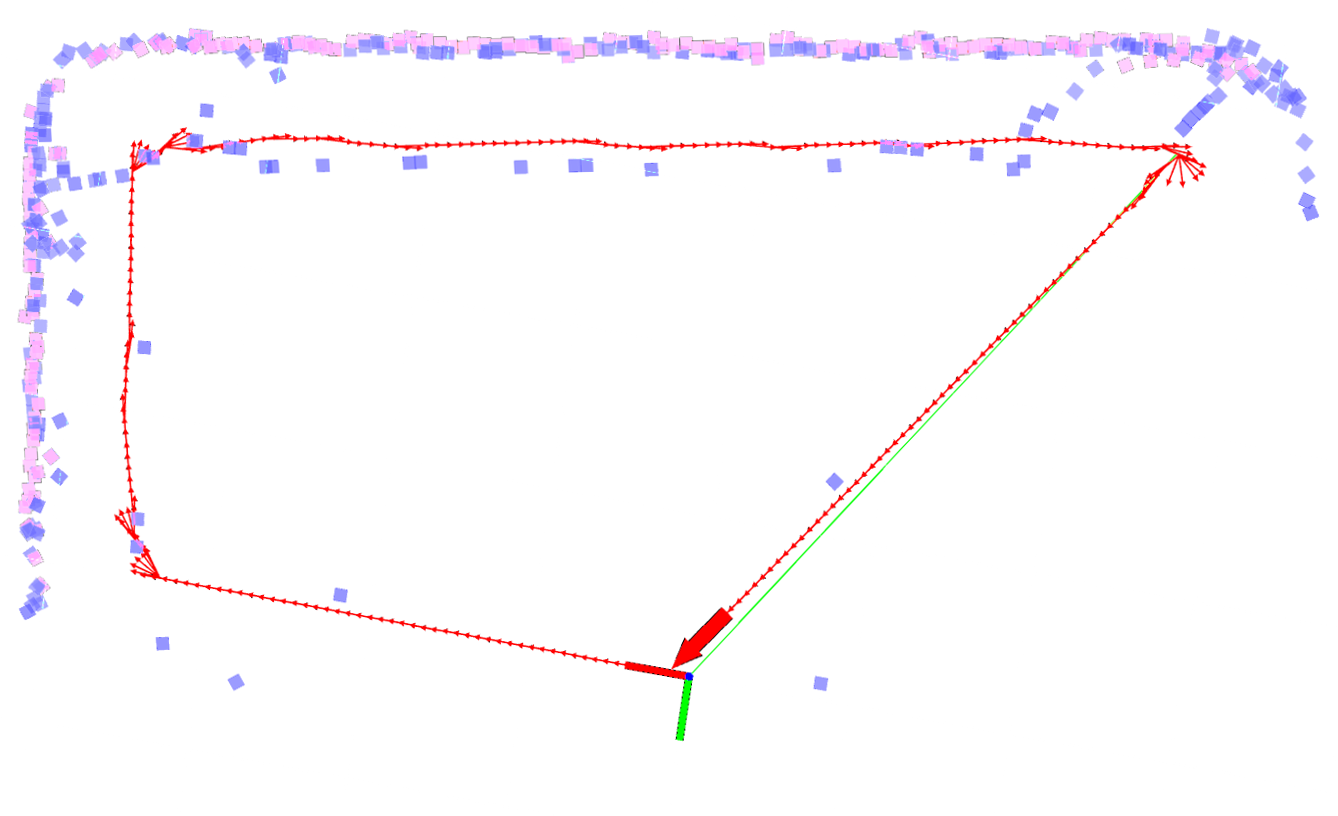
\includegraphics[width=30em]{../assets/right-angle-calibration.png}
    \caption{The robot starts in the centre of an empty squre box, heads towards the wall, turns to follow the wall, then turns the box corner which is $90$ \degree, follows the wall for some more time, and heads to its starting position (where it stops).}
  \end{center}
\end{figure} 


%       ^v^v^v^v^v^v^v^v^v^v^v^v^v^v^v^v^v^v^v^v^v^v^v^v^v^v^v^v^v^v^v^v^v^v^v^

\newpage
\section{Plotting}
\label{Plotting}

At each epoch in the control loop, a Pose and sensor-activation array is published to a Redis channel.
If the goal has changed, it is also published to a separate channel. 

%TODO remove repeated M-line description

In the case of \textit{Bug2} this goal line will be the so-called \textit{m-line}, representing a 
straight path the return algorithm will attempt to take. As the Redis instance is network-accessible 
and running as it's own process, this prevents any rendering or plotting activity from stalling or 
slowing the control loop. This also keeps loop run-time consistent, and allows the rendering to
be done on a separate computer.

In the case of using RViz to render our data, \texttt{data.py} contains code for 
subscribing to all the Redis channels the control loop will publish to and exposing 
ROS Topics for the same data that can be picked up by RViz or any other ROS compatible 
program.

The data received from the control loop is raw sensor data, that requires both conversion to
actual distance data and translation from the Khepera's frame of reference to the global frame.
The activation to distance conversion was done using an equation from an equation solver and 10
samples of \textit{distance, activation} pairs.

\begin{figure}[h]
  \begin{center}
    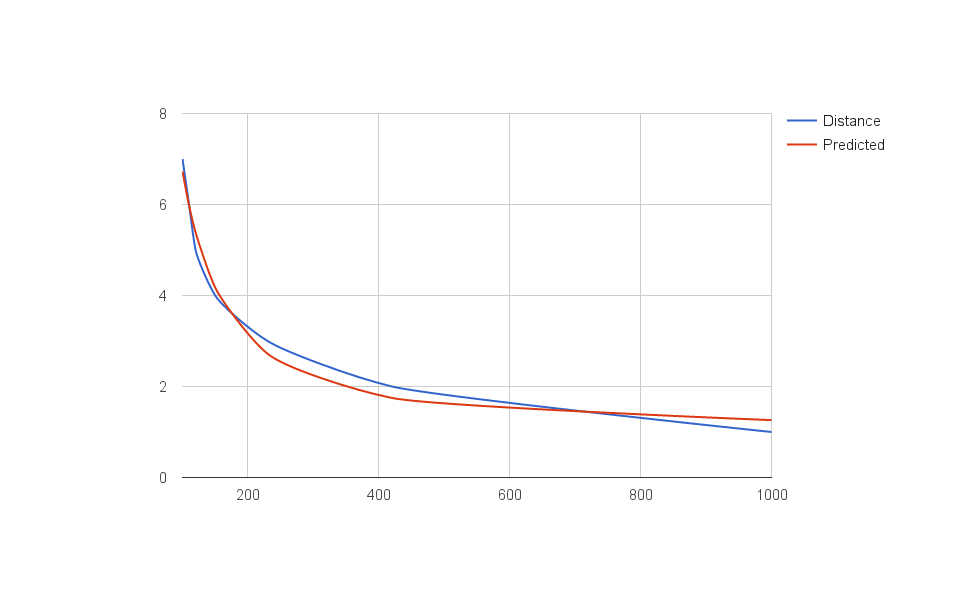
\includegraphics[width=30em]{../assets/plots/sensor-equation.png}
  \end{center}
  \begin{equation}
    S = 1.074519 + 
    \frac{9.502961}
         {(1 + \frac{\alpha}{70.42612}^{69.9039})^{0.02119919}}
  \end{equation}
  \caption{Solved equation translation betweek $S$, the distance, and $\alpha$, 
    the raw activation data of the sensor.}
\end{figure}

The reference pane transformation is performed by a ${3\times3}$ matrix, rotating and translating
onto the global reference pane.

\subsection{mapping}

A simple map is evolved as the Robot explores it's environment. We can derive solids in the environment
from the distance sensor readings, by discarding distances above a given threshold but persisting a
\textit{voxel} for any readings that are closer than this threshold.

\begin{figure}[h]
  \begin{center}
    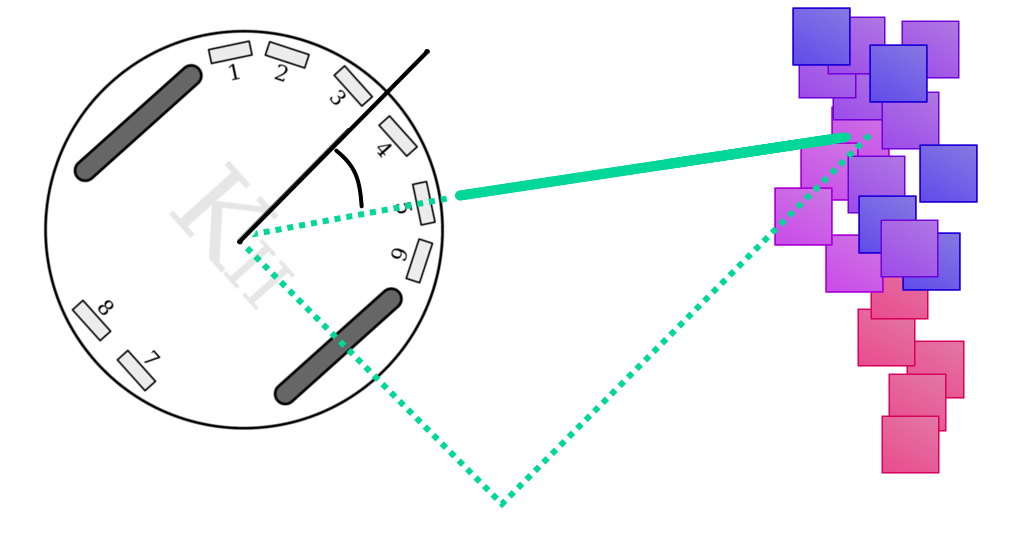
\includegraphics[width=30em]{../assets/khepera-wall.png}
  \end{center}
  \caption{\textbf{Left:} Illustration showing voxels colourised by proximity (red closer) and their
    relation to the Khepera robot. \textbf{Right:} Part of the map evolved, showing voxels and a
    red odometry trail of poses}
\end{figure}

%ANGUS - the voxel diagram is backwards and very unclear, just make it a slope in front of the robot or something... no need for the trigonometry

%TODO fix it

\begin{figure}[h]
  \begin{center}
    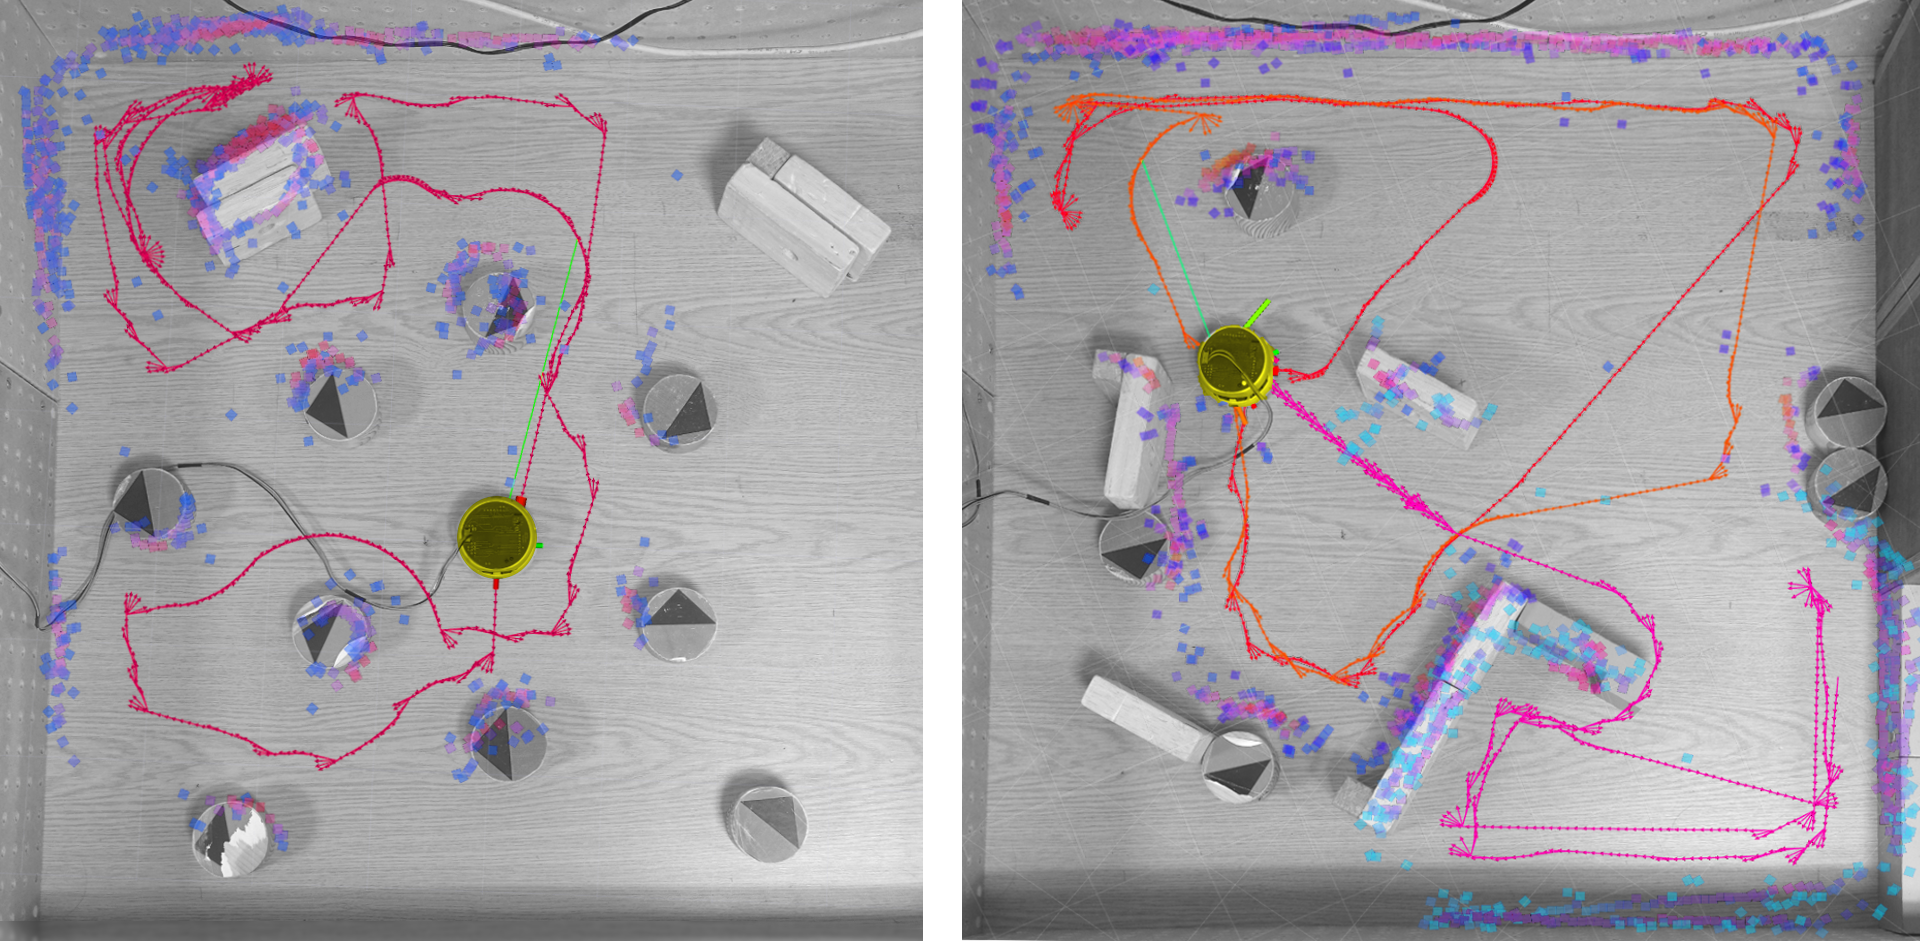
\includegraphics[width=38em]{../assets/merged_top_fig.png}
  \end{center}
  \caption{Top-down hybrid Rviz plot and photograph, showing \textbf{left} a long duration (~1m)
    exploration, and \textbf{right} multiple explorations and returns in the same environment, where a
    different route was taken each time.}
\end{figure}

%       ^v^v^v^v^v^v^v^v^v^v^v^v^v^v^v^v^v^v^v^v^v^v^v^v^v^v^v^v^v^v^v^v^v^v^v^
\newpage
\section{Return Algorithm}
\label{Return Algorithm}

Since Task 2 only mentions odometry and mapping is only mentioned in Task 3, we assumed that we should
be able to return to the start position of the robot ${(0,0)}$ (the goal) with using only IR sensors for avoiding obstacles
and odometry for pose calculations. 


%       ^v^v^v^v^v^v^v^v^v^v^v^v^v^v^v^v^v^v^v^v^v^v^v^v^v^v^v^v^v^v^v^v^v^v^v^

\subsection{Research}

Through researching for algorithms that would only use the end (and knowing the current) position for navigation, 
found the so called Bug algorithms as the are insect inspired. Bug 2 is the robuts and 
(on average) the most efficient out of the three mentioned bug algorithms. 
Hence, it was chosen to be implemented.


%       ^v^v^v^v^v^v^v^v^v^v^v^v^v^v^v^v^v^v^v^v^v^v^v^v^v^v^v^v^v^v^v^v^v^v^v^


\subsection{Method Chosen}

The Bug 2 algorithms is quite easy conceptually. The assumptions it needs to work properly can be simplified to:

\begin{enumerate}

	\item Known direction to goal and robot can measure distance between points
	\item Be in a bounded workspace with a finite number of finitie size objects

\end{enumerate}

Hence, we satisfy these assumptions by having odometry and a global frame of reference as well 
as a square box arena with physical obstacles.

The algorithm is:

\begin{enumerate}

	\item Head toward goal on the m-line - the straight line drawn from the start point to the goal
	\item if an obstacle is in the way, follow it until you encounter the m-line again closer to the goal
	\item Leave the obstacle and continue toward the goal

\end{enumerate}

Below is the a demonstation of the algorithm in a diagram

\begin{figure}[h]
  \begin{center}
    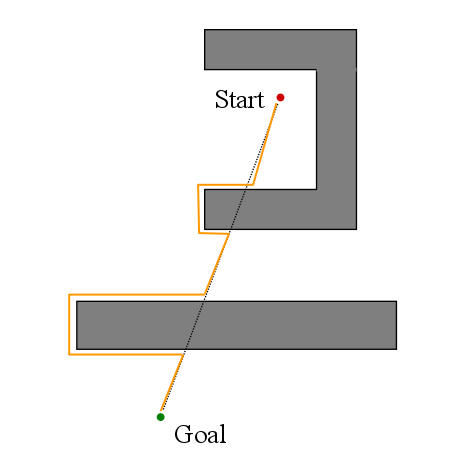
\includegraphics[width=30em]{../assets/bug-algorithm-diagram.png}
    \caption{The Bug 2 basic operation diagram. The Goal is where it is trying to go to and the Start is where it starts said journey to. The straight line between them is the M-line.}
  \end{center}
\end{figure} 


%       ^v^v^v^v^v^v^v^v^v^v^v^v^v^v^v^v^v^v^v^v^v^v^v^v^v^v^v^v^v^v^v^v^v^v^v^

\subsection{Integration}

The algorithm is activated after $\approx 30$ seconds of exploration\cite{task1_report} and after
activation is the leading algorithm unless on of the following are true for that control loop iteration:

\begin{enumerate}	

	\item The reactive control (getting "unstuck"\cite{task1_report})activates - reactive avoidance algorithm is in control
	\item There is a miscalculation for the new speeds and they robot may try to drive towards the wall it is following - exploration algorithm is in control

\end{enumerate}
%TODO put all references

The second point can occur if M-line recomputation occurs as described in \textit{M-line Replanning}

Below is a diagram showing how the controlling $3$ algorithm (ractive avoidance, exploration and return algorithm)
is chosen at every iteration of the loop (starting from the start marker). Before the 30 second mark robot
performs exactly as for Task 1, after that the "boredom"\cite{task1_report} is disabled. Please note
that unlike in the report for Task 1, here the collistion voidance is regarded as a separate algorithm from the
wall following, forward driving and "boredom" ("exploration algorithm") one

The following is a representation of the algorithm in a state diagram form:
\begin{figure}[h]
  \begin{center}
    \includegraphics[width=30em]{../assets/control-choice-diagram.png}
    \caption{Control algorithm choice in a state diagram form.}
  \end{center}
\end{figure} 


%       ^v^v^v^v^v^v^v^v^v^v^v^v^v^v^v^v^v^v^v^v^v^v^v^v^v^v^v^v^v^v^v^v^v^v^v^

\subsection{Needed Alterations}
\label{Needed Alterations}

%TODO mention that it sometimes gets stuck etc

However, the implementation is much less trivial than the higher level description. It it had 
to be altered due to problems that became evident during testing \textit{\S\ref{Experimental 
Results} Experimental Results} and are generalized below.

\subsubsection{Thresholding}

%       ^v^v^v^v^v^v^v^v^v^v^v^v^v^v^v^v^v^v^v^v^v^v^v^v^v^v^v^v^v^v^v^v^v^v^v^


the first problem is that due to imperfect encoders, wheel slippage, odometry drift as well as not
beign able to sample odometry more often than every $20$ ms\cite{khepera_manual} (due to sequential 
reads of IR being in the same loop. Moreover, one must remember odometry fomulas used are only approximations.

Hence, all odometry and position-related calculations can not be strict equalities to compensate 
for the error the above introduces. Hence, all values are considered "on-point" as long as the 
fall within $\pm$ threshold of ideal value. Some thresholds are several centimeters.


%       ^v^v^v^v^v^v^v^v^v^v^v^v^v^v^v^v^v^v^v^v^v^v^v^v^v^v^v^v^v^v^v^v^v^v^v^

\subsubsection{M-line Replanning}


Testing also revealed that about $1/15$ times the claculations of the approach angle to the goal would 
fail and be 180 \degree more than the real value. Many attampts were made to trace down the bug, however,
none were successful. Hence, we made an alteration to the Bug 2, so if it is in free space (not following 
walls or beign "unstuck"\cite{task1_report}) and it goes away from the last detected m-line segment for more
than a threshold value, we recompute the approach vector to the goal.

This revealed another bug that was left over from task 1 as in the wall following was state-based and sometimes
a spike in sensor readings made it seem that the tobot left the wall and was in free space, recomputing the M-line
wrongly even if it continued to follow the wall. 


This was countered by introducing another distance check into the Bug algorithm, to check if we could still 
theoretically follow the wall, in which case the threshold at which we would recompute the M-line was several 
times larger than the one for recom[uting in free space. Hence, even if robot gets stuck in a particular scenarion, 
there should be very few edge cases wher it will get trapped and continue reocmputing the M-line, getting itself stuck again.
Altering the two constants for M-line recomputing is what was also done durting testing to minimize said edge cases.


Below if the final form of the return algorithm that we have used

\begin{figure}[h]
  \begin{center}
    \includegraphics[width=30em]{../assets/return-algorithm.png}
    \caption{The return algorithm in a state diagram form where the oval shape is the conditional action done before going to Bug 2 algorithm. That action replans the M-line.}
  \end{center}
\end{figure} 



%       ^v^v^v^v^v^v^v^v^v^v^v^v^v^v^v^v^v^v^v^v^v^v^v^v^v^v^v^v^v^v^v^v^v^v^v^

\section{Experimental Results}
\label{Experimental Results}


%TODO insert results


%       ^v^v^v^v^v^v^v^v^v^v^v^v^v^v^v^v^v^v^v^v^v^v^v^v^v^v^v^v^v^v^v^v^v^v^v^


\section{Discussion \& Possible Improvements}

\label{Results}


%TODO say what is long and waht is short
Various system implementation methods were reasrched, best ones chosen, implemented and 
tested in both sprase and dense environment for both short and long periods of time. It
should be noted that this time was proportional to the exploration time set.

The more the robot drove around, the more the odometry drift increased and the further it got from the 
start point, while thinking it stopped at the spot it started at. It was also noted that the more 
turns the robot had to do the more the drift became. However, the path that was taken by the robot,
the angles of the turns and distances were identified very accurately. Hence, even though it worked very 
well in highly dense environments, the above errors were virtually unnoticeable in sparse environments.

The plotting worked wonders and not only allowed us to properly test our odometry as well as return algorithm,
but also visualize the environment in a highly comprehensible and inforamtive way. Moreover, it uses a separate
data server, which means if the main program crashes the data is not lost. Furthermore, we have derived a 
distance formula for the distance to the obstacle based on the IR values. Lastly, the way it was developed 
allows an easy transition towards SLAM (hint hint).

Lastly, the subsumptious hybrid architecture that was developed between the three algorithms (as described
before) worked very well and allowed the robot to properly switch between behaviors. The reutrn algorithm's precision
depends on positioning errors, hence, it's errors also come from odometry. However, it worked with a
very high sucess rate, getting stuck in only edge cases where it would be trapped in a very deep pocket which
protruded almost towards the goal and had very logn walls until the robot could escape. Hence, that is the only case
when we had a failure rate and it was $50\%$. %TODO check values

\label{Discussion}

Attempts to correct the algorithmic flaws were made as per above and in \textit{\S\ref{Needed Alterations} Needed Alterations}
and could yield better results if wall sticking is fixed to where the approach was used
would not be needed, leaving the algorithm as closely unchanged to Bug 2.

Lastly, another improvement would be more accurate encoders which are not magnetic as before repairs
our robot was swirving to the side and the encoders were not detecting that, therefore we might predict
that the main source of drift is said poor detection and the approximations that are used for formulas
to compute the pose.


However, we would consider it a sucessful odometric, plotting and returning hybrid subsumptious 
mobile autonomous system. 


%       ^v^v^v^v^v^v^v^v^v^v^v^v^v^v^v^v^v^v^v^v^v^v^v^v^v^v^v^v^v^v^v^v^v^v^v^

\newpage
\begin{thebibliography}{8}

%ANGUS - which one of these is the BUG one ?

\bibitem{principlesrobot}
\par{Principles of Robot Motion: Theory, Algorithms, and Implementation \S2.1}\\
\textit{Howie Choset}

\bibitem{Redis}
\par{Redis is an open source (BSD licensed), in-memory data structure store, used as database, cache and message broker. It supports data structures such as strings, hashes, lists, sets, sorted sets with range queries, bitmaps, hyperloglogs and geospatial indexes with radius queries.}\\
\textit{http://redis.io}

\bibitem{ROS}
\par{The Robot Operating System (ROS) is a flexible framework for writing robot software. It is a collection of tools, libraries, and conventions that aim to simplify the task of creating complex and robust robot behavior across a wide variety of robotic platforms.}\\
\textit{http://www.ros.org/}

\bibitem{runge_kutta} 
\par{Fourth order Runge - Kutta algorithm for pose estimation} \\
\textit{https://www.cs.cmu.edu/afs/cs.cmu.edu/academic/class/16311/www/s07/labs/NXTLabs/Lab\%203.html}

\bibitem{odo_used} 
\par{Princeton University lecture on Autonomous Robot Navigation with odometry formulas and their deriviation from geometry and trigonometry. These formulas are devised specifically for differential drive robots} \\
\textit{https://www.cs.princeton.edu/courses/archive/fall11/cos495/COS495-Lecture5-Odometry.pdf }

\bibitem{odo_calibration} 
\par{The Technic Gear website article dealign with differential drive robot odometry calculations} \\
\textit{http://thetechnicgear.com/2014/06/howto-calibrate-differential-drive-robot/}

\bibitem{khepera_paper} 
\par{A paper on Experimental Odometry Calibration of the Mobile Robot Khepera II Based on the Least-Squares Technique from which we took inspiration on calibration and confirmation we are doing odometry in the right fashion} \\
\textit{http://ieeexplore.ieee.org/stamp/stamp.jsp?arnumber=1570321}

\bibitem{khepera_manual} 
\par{Khepera 2 user Manual containing all the fundamental information about the Khepera 2 robot, including information abotu encoders and their value meanings} \\
\textit{http://ftp.k-team.com/khepera/documentation/Kh2UserManual.pdf}

\bibitem{task1_report} 
\par{Our Task1 solution and report} \\
\textit{Angus Pearson, Jevgenij Zubovskij}





\end{thebibliography}


\begin{appendices}
\section*{Appendix}
\subsection{Code Listings}
\lstinputlisting[language=python]{../../main.py}
\lstinputlisting[language=python]{../../data.py}
\lstinputlisting[language=python]{../../state.py}
%ANGUS - where is nav state...... XD
\lstinputlisting[language=python]{../../bug_state.py}
\lstinputlisting[language=python]{../../bug_algorithm.py}
\lstinputlisting[language=python]{../../navigation_algorithm.py}
\lstinputlisting[language=python]{../../odometry_algorithm.py}
\lstinputlisting[language=python]{../../odometry_state.py}
\lstinputlisting[language=python]{../../constants.py}
\end{appendices}


\end{document}
